\section{Gegevensmodel}
\subsection{Data format}
Het dataformaat van de u-blox is NMEA, NMEA is een standaardprotocol voor het
weergeven van GPS-data. Dit ziet er zo uit: \\
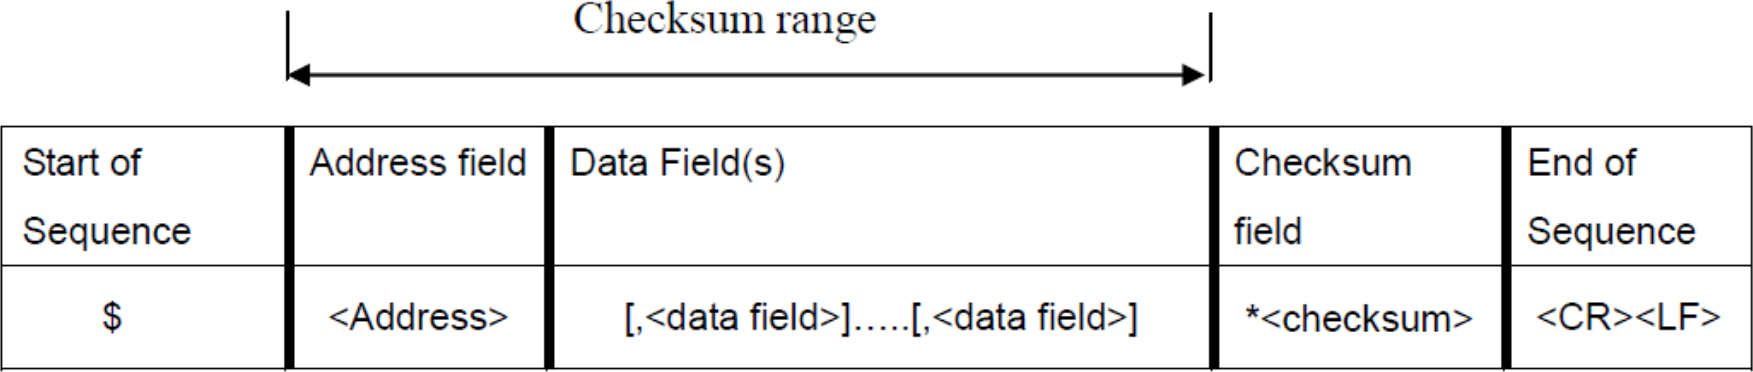
\includegraphics[width=\textwidth]{technical/nmea}
\\Hierbij is het adres veld in het formaat ``aaccc'', waarbij ``aa'' het
Talker ID is en ``ccc'' het soort bericht. Velden zijn gesepareerd met
een ``,''.
\citep{Navspark}\\\\
Het belangrijkste deel van dit format zijn de GNS-berichten
(GNSS-data). Deze berichten zien er als volgt uit:\\
\texttt{\$GPGNS,091547.00,5114.50897,N,00012.28663,W,AA,10,0.83,111.1,45.6,,,V*71}
\\\\
De velden houden in:
\\\\
\begin{tabularx}{\textwidth}{| l | l | l | l | X |}
    \hline
    \textbf{Veld} & \textbf{Naam} & \textbf{Formaat} & \textbf{Voorbeeld} & \textbf{Beschrijving}          \\ \hline
    0             & xxGNS         & string           & \$GPGNS            & GNS ID (xx = current Talker)   \\ \hline
    1             & Tijd          & hhmmss.ss        & 091547.00          & Tijd (UTC)                     \\ \hline
    2             & Latitude      & ddmm.mmmmm       & 5114.50897         & Latitude (graden en minuten)   \\ \hline
    3             & NS            & character        & N                  & Noord/Zuid                     \\ \hline
    4             & Longtitude    & dddmm.mmmmm      & 00012.28663        & Longtitude (graden en minuten) \\ \hline
    5             & EW            & character        & E                  & Oost/West                      \\ \hline
    6             & posMode       & character        & AA                 & Positionering mode             \\ \hline
    7             & numSV         & numeric          & 10                 & Aantal satellieten             \\ \hline
    8             & HDOP          & numeric          & 0.83               & Horizontal dilution precision  \\ \hline
    9             & alt           & numeric          & 111.1              & Hoogte boven zeeniveau         \\ \hline
    10            & sep           & numeric          & 45.6               & Geoïde separatie               \\ \hline
    11            & diffAge       & numeric          & -                  & Leeftijd correctie             \\ \hline
    12            & diffStation   & numeric          & -                  & ID GPS-correctie station       \\ \hline
    13            & navStatus     & character        & V                  & Navigatie Status               \\ \hline
    14            & cs            & hexadecimal      & *71                & Checksum                       \\ \hline
    15            & <CR><LF>      & character        & -                  & Carriage Return                \\ \hline
\end{tabularx}
\citep[p. 116]{UBlox8}\\
Een ander deel van de data die we mogelijk gaan gebruiken is:
\texttt{\$GPGBS}. \texttt{\$GPGBS} bevat de afwijking van de data bij u-blox
DGPS-toestellen.
\citep[p. 111]{UBlox8}

De uiteindelijke data die we gaan gebruiken is:
ID, Tijd (UTC), Latitude, Longtitude en Altitude

Voor het referentiestation komt hier nog bij:
error Latitude, error Longtitude en error Altitude

\subsection{Database}
\label{sec:database}

De verstuurde data zal worden bijgehouden in een SQL-database. Tijdens het testen
zal dit op een extern gehoste server zijn.
Wanneer er een eigen LoRa gateway met de markers gebruikt wordt zal deze database
een lokaal, offline, systeem zijn. De data zal dan naar een centrale database
worden verstuurd wanneer er een goede internetverbinding is.

De tabel met de meetpunten zal de volgende kolommen bevatten:
\begin{itemize}
    \item Meetpunt ID
    \item Marker nummer
    \item Latitude
    \item Longitude
    \item Tijdstip van registratie
\end{itemize}

Verder zal er een tabel zijn met de percelen, deze bevat de kolommen:
\begin{itemize}
    \item Perceel ID
    \item Perceelnummer
\end{itemize}

Om de percelen en meetpunten aan elkaar te koppelen zal er een koppeltabel komen:
\begin{itemize}
    \item Perceel ID
    \item Volgnummer
    \item Meetpunt ID
\end{itemize}
